%
% Design, XIN YUAN, 2020
%

\chapter{W~语言设计}

如前面所述,~W~语言兼具通用底层语言和高级应用语言的特征。因此
本章详细描述语言的语法设计。

\section{语言的生成目标}

该语言的生成目标是操作系统上用户态的可执行映像以及动态装载映像。
对于驱动级系统程序,则是另外一类和具体操作系统有关的核心态映像。
目前主要考虑~Windows~操作系统和~X~系列操作系统。生成的各类映像
应该包含程序代码和各类数据~(~资源~)~,并且能够被从外部访问。

根据设计模式的不同,动态映像可包含普通的程序码~(~通过引出函数
访问~)~以及资源~(~通过资源编号访问~)~和组件对象~(~通过接口规范
访问~)~。

该语言也可以像~VBA,JavaScript,VBScript~一样成为宿主应用程序下的
脚本语言被宿主控制调用以解释或者虚拟机或者本地机器码方式执行。

\section{语言的实现步骤}

为了使语言可以跨各种硬件平台和操作系统,将使用如下三步来完成最终
的编译器和链接器。
\begin{enumerate}
\item{用~C~语言在~windows~和~IA32~平台下实现~W~语言的子集}

该步骤使用~VC~作为编译工具实现~W~语言的一个子集,即面向过程的
部分。实现的编译器和链接器均为~windows~和~IA32(Intel Architecture)~
下运行的程序。采用这样的设计是为了最终能利用~W~语言本身的跨平台
特性来编写最终的多平台编译器。

\item{用~W~语言在~windows~和~IA32~平台下实现多平台的~W~语言}

这个步骤使用~W~语言的一个面向过程的子集,编写~W~语言本身的编译器
和链接器。该步骤编写时就要设计为能生成不同的硬件架构下的机器码
以及不同操作系统下的可执行映像。

\item{用~W~语言编写库并生成各平台下的编译器和链接器}

该步骤使用~W~语言编写运行库和开发工具。

\end{enumerate}

\chapter{W~语言子集基本要素}

~W~语言的子集是一个面向过程的语言。因此它和~C~语言类似。它的
基本要素包括:

\begin{itemize}
\item{数据基本类型}

这里设计实现了一些基本的通用数据类型,与具体机器无关。基本数据
类型包括:值类型和引用类型。

\item{变量和常量}

设计实现了变量和常量的定义和使用。

\item{类型转换}

设计了隐式类型转换和显式类型转换。

\item{表达式}

设计了操作符、算术表达式、赋值表达式、关系表达式、逻辑表达式、位
运算以及其他特殊的表达式。

\item{流程控制}

设计了顺序结构、条件结构、循环结构。以及条件编译。

\item{编译单元的结构}

设计了编译单元的语法结构。

\end{itemize}

\section{数据基本类型}

%
% Basic Data Types, XIN YUAN, 2020
%

数据类型分为值类型和引用类型两种。

\subsection{值类型}

变量是存储信息的基本单元;是计算机内存中的一个存储空间。

值类型分为几下几种:

\begin{itemize}
\item{简单类型}
\item{结构类型}
\item{枚举类型}
\item{联合体和位段类型}
\end{itemize}

简单类型即纯量类型,是直接由一系列元素构成的类型。包括整数、
布尔、字符、实数四种。

\subsubsection{整型}

计算机上的整数是有范围的。表~\ref{tab_int}~ 就是整数类型的表示。

\begin{table}[h]
  \centering
  \caption{整数类型}\label{tab_int}
  \vspace{1.5ex}
\begin{tabular}{|l|l|l|}
  \hline
  % after \\: \hline or \cline{col1-col2} \cline{col3-col4} ...
  \textbf{数据类型} & \textbf{特征} & \textbf{取值范围} \\
  \hline\hline
  char & 有符号~8~位整数 & -128~127 \\
  \hline
  uchar & 无符号~8~位整数 & 0~255 \\
  \hline
  short & 有符号~16~位整数 & -32768~32767 \\
  \hline
  ushort & 无符号~16~位整数 & 0~65535 \\
  \hline
  long & 有符号~32~位整数 & -2147483648~2147483647 \\
  \hline
  ulong & 无符号~32~位整数 & 0~4294967295 \\
  \hline
   &  & -9223372036854775808 \\
  \raisebox{1.3ex}[0pt]{int64} & \raisebox{1.3ex}[0pt]{有符号~64~位整数}
  & ~9223372036854775807 \\
  \hline
  uint64 & 无符号~64~位整数 & 0~18446744073709551615 \\
  \hline
  int128 & 有符号~128~位整数 & $-2^{63}$~$2^{63}-1$ \\
  \hline
  uint128 & 无符号~128~位整数 & $0$~$2^{64}-1$ \\
  \hline
\end{tabular}

\end{table}

此外定义两个关键字:~int~和~uint~,用来表示机器字长的整数。不同
的机器通用寄存器的字长不同,利用这两个类型的变量可以表示不同目标
机器上的通用寄存器整数,从而实现跨硬件平台。

整数的内存表示只需要注意不同硬件上的大端和小端问题。

以上整数的正则表达式为:

\newcommand{\clrsmall}[1]{\textcolor{magenta}{#1}}
\newcommand{\clrbig}[1]{\textcolor{blue}{#1}}

\begin{Verbatim}[frame=single, commandchars=*()]
    *clrsmall(digit)     [0-9]
    *clrsmall(hex_digit) [0-9a-fA-F]
    *clrbig(TK_PINUM)   {digit}+
    *clrbig(TK_PHEXNUM) 0[xX]{hex_digit}+
    *clrbig(TK_KEY_CHAR)     "char"
    *clrbig(TK_KEY_UCHAR)    "uchar"
    *clrbig(TK_KEY_SHORT)    "short"
    *clrbig(TK_KEY_USHORT)   "ushort"
    *clrbig(TK_KEY_LONG)     "long"
    *clrbig(TK_KEY_ULONG)    "ulong"
    *clrbig(TK_KEY_INT64)    "int64"
    *clrbig(TK_KEY_UINT64)   "uint64"
    *clrbig(TK_KEY_INT128)   "int128"
    *clrbig(TK_KEY_UINT128)  "uint128"
    *clrbig(TK_KEY_INT)      "int"
    *clrbig(TK_KEY_UINT)     "uint"
\end{Verbatim}

\subsubsection{布尔型}

布尔型是用来表示“真”和“假”的概念的。采用关键字~true~和~false~来
表示。和~C~与~C++~不同,~true~不能用其他非零值代替。整数类型不能
转换为布尔型。用关键字~bool~表示该数据类型。实现的方式是针对同一
个作用域,将所有~bool~变量集中到一个或多个~int~变量,每个~bool~变
量占用一个位。

正则表达式:

\begin{Verbatim}[frame=single, commandchars=\\\{\}]
    \textcolor{blue}{TK_KEY_BOOL}   "bool"
    \textcolor{blue}{TK_KEY_TRUE}   "true"
    \textcolor{blue}{TK_KEY_FALSE}  "false"
\end{Verbatim}

\subsubsection{字符型}

字符分为~char~和~wchar~两种,分别表示~ANSI~字符和~UNICODE~字符。
其中~wchar~的位数根据系统的不同而不同。~Windows~下是~16~位的,某些
~X~系统下是~32~位的。它们需要显式转换为其他类型。

如下代码对字符赋值:

\lstsetwlang

\ttfamily
\begin{lstlisting}
    char c = 'A';
    wchar c = L'A';
    char c = '\x05';
    wchar c = L'\x05';
    wchar c = '\x0032';
\end{lstlisting}
\CJKfamily{song}

其中前缀~L~表示其后字符为~UNICODE~字符;~$\backslash$x~后跟一个~16~
进制数表示字符。

转义符~``$\backslash$''~用来表示特殊的控制字符,如表~\ref{tab_esc}~
所示:

\begin{table}[h]
  \centering
  \caption{转义符}\label{tab_esc}
  \vspace{1.5ex}
\begin{tabular}{|l|l|}
  \hline
  % after \\: \hline or \cline{col1-col2} \cline{col3-col4} ...
  \textbf{转义符} & \textbf{含义} \\
  \hline\hline
  $\backslash$' & 单引号 \\
  \hline
  $\backslash$'' & 双引号 \\
  \hline
  $\backslash\backslash$ & 反斜杠 \\
  \hline
  $\backslash$0 & 空字符 \\
  \hline
  $\backslash$a & 感叹号 \\
  \hline
  $\backslash$b & 退格 \\
  \hline
  $\backslash$f & 换页 \\
  \hline
  $\backslash$n & 新行 \\
  \hline
  $\backslash$r & 回车 \\
  \hline
  $\backslash$t & 水平~tab~ \\
  \hline
  $\backslash$v & 垂直~tab~ \\
  \hline
  $\backslash$x & 后面的数字是~16~进制数 \\
  \hline
\end{tabular}

\end{table}

正则表达式:

\begin{Verbatim}[frame=single, commandchars=*\#\~]
    *clrsmall#ansi_char~      ([^'\"\n]|\\(['\"\\0abfnrtv]|
                             x{hex_digit}{hex_digit}))
    *clrsmall#wide_char~      (\\x{hex_digit}{hex_digit}
                              {hex_digit}+
                             |[x80-xff][x00-xff])
    *clrbig#TK_KEY_WCHAR~   "wchar"
    *clrbig#TK_CONST_CHAR~  '{ansi_char}'
    *clrbig#TK_CONST_WCHAR~ ((L'{ansi_char})|('{wide_char}))'
\end{Verbatim}

\subsubsection{实型}

实数类型包括浮点和十进制数两种类型。

\textbf{浮点类型}

浮点包括单精度~(float)~,双精度~(double)~和长精度~(longdbl)~三种
类型。计算机对浮点数的运算速度大大低于对整数的运算速度。

\begin{itemize}
\item{单精度}

占~32~位,取值范围:~$\pm 1.5\times 10^{-45}$~到
~$\pm 3.4\times 10^{38}$~,小数精度~7~位数。

内存格式:待补充。。。。。。
无效数的表示:

\item{双精度}

占~64~位,取值范围:~$\pm 5.0\times 10^{-324}$~到
~$\pm 1.7\times 10^{308}$~,小数精度~15~到~16~位数。

内存格式:待补充。。。。。。
无效数的表示:

\item{长精度}

占用~80~位,

内存格式:待补充。。。。。。
无效数的表示:

\end{itemize}

\textbf{十进制类型}

十进制数~(decimal)~主要用来表示金融和货币的数字计算。它是高精度、
~128~位的数字类型,表示范围为~$\pm 1.0\times 10^{-28}$~到
~$\pm 7.9\times 10^{-28}$~,有效数字~28~至~29~位。运算结果准确到
~28~个小数位。

十进制类型的计算机内存格式:待补充。。。。。。
无效数的表示:

实数常量代码表示:

\ttfamily
\begin{lstlisting}
    float a = 1.0f;
    double a = 1.0;
    longdbl a = 1.0ld;
    decimal a = 1.0m;
\end{lstlisting}
\CJKfamily{song}

其中后缀~f~表示单精度浮点数,~ld~表示双精度浮点,~m~表示十进制数。

正则表达式:

\begin{Verbatim}[frame=single, commandchars=^\#\~]
    ^clrsmall#num_exp~      [eE][+-]?{digit}+
    ^clrsmall#float_num~    ({digit}+"."{digit}*({num_exp})?|
                       {digit}+{num_exp}|
                       "."{digit}+({num_exp})?)
    ^clrbig#TK_KEY_FLOAT~       "float"
    ^clrbig#TK_KEY_DOUBLE~      "double"
    ^clrbig#TK_KEY_LONGDBL~     "longdbl"
    ^clrbig#TK_KEY_DECIMAL~     "decimal"
    ^clrbig#TK_CONST_PFLOAT~    {TK_PINUM}f|{float_num}f
    ^clrbig#TK_CONST_PDOUBLE~   {float_num}
    ^clrbig#TK_CONST_PLONGDBL~  {TK_PINUM}ld|{float_num}ld
    ^clrbig#TK_CONST_PDECIMAL~  {TK_PINUM}m|{float_num}m
\end{Verbatim}

\subsubsection{结构类型}

结构将一系列变量组织成一个单一的实体。每个变量称为结构的成员。
结构用~struct~来声明,如下所示:

\ttfamily
\begin{lstlisting}
    struct PhoneBook
    {
        int a;
        int b;
    }
    PhoneBook t;
\end{lstlisting}
\CJKfamily{song}

~t~就是一个结构类型的变量。结构的成员全部是~public~类型,即可以
通过变量名加上``~.~''号,再加上成员名称来访问:

\ttfamily
\begin{lstlisting}
    t.a = 2;
\end{lstlisting}
\CJKfamily{song}

结构的成员类型可以是前面的简单类型,也可以是结构体、联合体、枚举
或位段。结构体内部可以嵌套定义结构体、联合体、枚举和位段,其作用域
仅限于结构体内部。

正则表达式:

\begin{Verbatim}[frame=single, commandchars=^\#\~]
    ^clrsmall#letter~   [a-zA-Z_]
    ^clrbig#TK_KEY_STRUCT~  "struct"
    ^clrbig#TK_KEY_PRIVATE~ "private"
    ^clrbig#TK_KEY_PUBLIC~  "public"
    ^clrbig#TK_IDENTIFIER~  {letter}({letter}|{digit})*
    ^clrbig#TK_LCURLY~  "{"
    ^clrbig#TK_RCURLY~  "}"
    ^clrbig#TK_COMMA~   ","
    ^clrbig#TK_SEMI~    ";"
\end{Verbatim}

\subsubsection{枚举类型}

枚举~(enum)~为一组在逻辑上密不可分的整数值提供便于记忆的符号。可
如下声明:

\ttfamily
\begin{lstlisting}
    enum WeekDay
    {
        Sunday, Monday, Tuesday, Wednesday, Thursday,
        Friday, Saturday
    }
    WeekDay day;
    day = Tuesday;
\end{lstlisting}
\CJKfamily{song}

注意:结构是由不同类型的数据组成的一组新的数据类型,结构类型的变量
的值是由各个成员的值组合而成的。枚举类型的变量在某个时刻只能取枚举
中某一个元素的值,如上面的~day~,它的值要么是~Sunday~,要么是
~Monday~或其他的星期元素。但它在一个时刻只能代表具体的某一天,不能
既是星期二,又是星期三。

默认枚举中每个元素类型都是~int~型,且第一个元素的值为~0~,后面的
每一个连续的元素的值按加~1~递增。在枚举中,也可以给元素直接赋值,
如下代码把星期天的值设为~1~,其后元素的值分别为~2~,~3~$\ldots$。

\ttfamily
\begin{lstlisting}
    enum WeekDay
    {
        Sunday=1, Monday, Tuesday, Wednesday, Thursday,
        Friday, Saturday
    }
\end{lstlisting}
\CJKfamily{song}

为枚举类型的元素所赋的值的类型限于~long~、~int~、~short~和~byte~等
整数类型。

正则表达式:

\begin{Verbatim}[frame=single, commandchars=^\#\~]
    ^clrbig#TK_KEY_ENUM~    "enum"
    ^clrbig#TK_EQ~          "="
\end{Verbatim}

语法:

\begin{Verbatim}[frame=single, commandchars=^\#\~]
    ^clrsmall#enumerator_def~
     : TK_KEY_ENUM TK_IDENTIFIER
       TK_LCURLY ^clrsmall#enumerator_list~ TK_RCURLY
     ;
    ^clrsmall#enumerator_list~
     : ^clrsmall#enumerator~
     | ^clrsmall#enumerator_list~ TK_COMMA ^clrsmall#enumerator~
     ;
    ^clrsmall#enumerator~
     : TK_IDENTIFIER
     | TK_IDENTIFIER TK_EQ ^clrsmall#const_expression~
     ;
\end{Verbatim}

\subsubsection{联合体和位段类型}

联合体类似于

\subsubsection{小结}

前述结构体的对齐,
联合体
位段对齐。

前述的几种类型定义的前面还可以跟关键字~private~和~public~,表明
该类型可否被其他平级作用域所引用。

前述结构体、联合体、位段的语法:

\begin{Verbatim}[frame=single, commandchars=^\#\~]
    ^clrsmall#struct_def~ :
\end{Verbatim}

\subsection{引用类型}

引用类型的变量指该变量不直接存储所包含的值,而是指向它所要存储的值。
它存储的是实际数据的引用地址。引用类型本身不能再有引用类型,即引用的
引用是不允许的。

引用类型包括直接定义、委托和数组。

\subsubsection{直接定义}

任何数据类型包括派生类型都可以定义对应的引用变量。但是引用类型本身
不能定义对应的引用类型。如果有类似的编程需求,则可以将引用类型定义
在结构中,然后使用结构的引用变量。

\ttfamily
\begin{lstlisting}
    ref int a = null;
    int b;
    ref int c = ref(b);
\end{lstlisting}
\CJKfamily{song}

和~C++~不同,~W~语言的引用可以指向空对象。~ref~是一个取引用的操作符,
它可取得变量的引用地址并赋值给引用变量。

正则表达式:

\begin{Verbatim}[frame=single, commandchars=^\#\~]
    ^clrbig#TK_KEY_NULL~   "null"
    ^clrbig#TK_KEY_REF~    "ref"
\end{Verbatim}

\subsubsection{委托}

在~C~和~C++~语言中,指针是它们最强有力的工具之一,同时又给他们带来
很多苦恼之处。因为指针指向的数据类型可能并不相同,如你可能把~int~
类型的指针指向一个~float~类型的变量,而这时程序并不会出错。若你
删除了一个不应该被删除的指针,程序就有可能崩溃。可见,滥用指针给
程序的安全性带来隐患。

正因为如此,在~W~语言中取消了取消了指针这个概念。并且用引用来替代。
尽管如此,为了使~W~语言能编写最底层的系统程序,如驱动程序,~W~语言
仍然提供了语法,使得引用可以象指针一样操作,本身也可以参加运算和被
强制转换。引用变量后也可以跟数组运算符号~[]~,因此可以当作数组名
处理。这样的代码是不安全的,因此会在编译时作特别的提示。

委托~(delegate)~相当于~C~语言中的函数指针原型。委托是类型安全的。
委托的声明类似一般的函数声明,前面加~delegate~关键字,如:

\ttfamily
\begin{lstlisting}
    delegate int MyDelegate();
\end{lstlisting}
\CJKfamily{song}

以上声明了一个~MyDelegate~类型,在使用中需要利用这个类型来定义
变量,并把合适的函数地址赋给它。委托变量只能和~int~变量相互
强制转换。

\ttfamily
\begin{lstlisting}
    MyDelegate d;
    public int NormalMethod()
    {
        return 0;
    }
    d = NormalMethod;
    d();
\end{lstlisting}
\CJKfamily{song}

正则表达式:

\begin{Verbatim}[frame=single, commandchars=^\#\~]
    ^clrbig#TK_KEY_DELEGATE~ "delegate"
\end{Verbatim}

\subsubsection{数组}

数组是进行批量处理数据的。数组是一组类型相同的有序数据。数组
按数组名、数据元素的类型和维数来进行描述。

在~W~语言子集中,我们只实现固定长度的数组。固定长度的数组
定义格式:
\begin{Verbatim}[frame=single, commandchars=^\#\~]
    non-array-type[dim_separators] array-instance-name;
\end{Verbatim}

例如:
\ttfamily
\begin{lstlisting}
    int[5] a;
\end{lstlisting}
\CJKfamily{song}

实现时将在栈上分配相应的内存。如果要动态分配内存,则使用
~walloc~函数,并将返回值赋给一个引用变量。如下所示:
\ttfamily
\begin{lstlisting}
    ref int a = walloc(3*sizeof(int)) as ref int;
\end{lstlisting}
\CJKfamily{song}

使用数组时,可以在~``[]''~中加入下标来取得对应的数组元素。
数组元素的下标是从~0~开始的。第一个元素对应的下标是~0~,以后
逐个增加。

数组可以是多维的。而一维数组用的最普遍。下面是一个例子:
\ttfamily
\begin{lstlisting}
    int[5] arr;
    for(int i = 0; i < 5; i ++)
        arr[i] = i * i;
\end{lstlisting}
\CJKfamily{song}

这个程序创建了一个有~5~个~int~型元素组成的数组,并逐个赋值
初始化。下面是多维数组的声明和例子:
\ttfamily
\begin{lstlisting}
    int[2,3]   a;
    int[4,2,3] b;
\end{lstlisting}
\CJKfamily{song}

和~C~语言不同的是,各维数在一个~``[]''~内指明,用逗号隔开。使用
多维数组时也使用相同的格式。其中第一个维数变化慢,最后一个元素
变化快。对于二维数组,第一维就是行数,第二维就是列数。在内存中
的存储布局是按行存储的。大于三维时,最后二维看成面,前面的维数
指定了后面的面阵,并顺序存储。例如前例中的三维数组,在内存中的
排列次序为:
\ttfamily
\begin{lstlisting}
    b[0, 0, 0]  b[0, 0, 1]  b[0, 0, 2]
    b[0, 1, 0]  b[0, 1, 1]  b[0, 1, 2]
    b[1, 0, 0]  b[1, 0, 1]  b[1, 0, 2]
    b[1, 1, 0]  b[1, 1, 1]  b[1, 1, 2]
    b[2, 0, 0]  b[2, 0, 1]  b[2, 0, 2]
    b[2, 1, 0]  b[2, 1, 1]  b[2, 1, 2]
    b[3, 0, 0]  b[3, 0, 1]  b[3, 0, 2]
    b[3, 1, 0]  b[3, 1, 1]  b[3, 1, 2]
\end{lstlisting}
\CJKfamily{song}

多维数组前面部分维数可以看成一个引用变量。例如前面例子中的~a~是
~$2\times 3$~的数组,那么可以把~a[0]~和~a[1]~都看成引用变量,同时
也是一维数组名,数组长度都是~3~。上述数组名~a~或者~a[0]~可以被
强制转化为基本类型的引用变量,从而可以象指针那样高效率地访问内存
数据。

注意:数组定义不能用~typedef~来取得它的别名。


\section{变量和常量}

%
% Variables, XIN YUAN, 2020
%

每一门编程语言都有自己对变量和常量的命名和使用方式。本节阐述变量
和常量的用途、如何对变量和常量命名、如何定义和初始化变量和常量。

\subsection{变量}

程序要对数据进行读写运算等操作,当需要保存特定的值或计算结果时,
就需要用到变量。在变量中可以存储各种类型的信息,如姓名、车票价格
和文件长度等。

计算机中的变量代表存储地址,变量的类型决定了存储在变量中的数值的
类型。变量的值可通过赋值和“++”或“--”运算符的运算被改变。

变量使用的重要原则是:先定义后使用。

变量可以在定义时被赋值,也可以在定义时不被赋值。定义时被赋值的
变量具有初始值,而定义时不被赋值的变量没有初始值。可以在其后的
代码中为这样的变量赋值。


\section{类型转换}

设计了隐式类型转换和显式类型转换。

\section{表达式}

设计了操作符、算术表达式、赋值表达式、关系表达式、逻辑表达式、位
运算以及其他特殊的表达式。

\section{流程控制}

设计了顺序结构、条件结构、循环结构。以及条件编译。

\section{编译单元的结构}


\chapter{类的设计原则}

利用~ATL/WTL~编程,就是基于面向对象的编程了。类是
主要的程序形式。在设计自己的类之前,请查看~MSDN~
以及~ATL/WTL~的源代码,看是不是已经有实现好的相同
功能的类和函数了,如果已经有了,就直接使用,没有
必要自己再去写一个。如果源代码中不存在,或者已经有
类似的类和函数但功能还不强,那么才需要自己去编写类
和函数,或者从现有的类派生以扩展功能。本章将介绍
如何设计高效的~WTL~类。

\section{WIN32~封装原则}



\section{窗口类的设计原则}

数据类和显示类的分离

用户控制
CWindowImpl 派生的模板类
一般功能的最终控制 再定制该模板类
空的表示直接使用模板类的功能。

利用现有标准控制 子类化 超类化
直接写可创建的窗口类

\section{其他原则}

模板编程
几种设计模式:
泛型

模板参数的特性较多,且每种模板参数的每种特性都可能需要定制
函数式 CWinTrait$<>$既是如此
特性类Trait

基类作为模板参数
派生类作为模板参数
其他?
什么时候用派生类模板参数 什么时候用特性类和特化、偏特化?
需讨论 一类类型所共有的特性;有点像接口纯虚类,肯定比它们
减少虚函数开销,区别是二进制代码上不可分离。
功能上的策略模式,使用派生类作模板参数,也减少了虚函数开销,
但同时它也能实现其他模式,即功能上能够被多重继承方式来扩展
宿主模块的功能,做到真正的砖块化

一般支持类 Mix-in class

类的层次结构 展开后形成新的类 导致运行时类库的庞大
要注意公共的代码
不涉及定制的模板参数的方法 放在一个无模板的
基类中 定制的放在派生类 模板中。减轻编译器的负担

虚函数设计仍可使用 减少虚函数 用于某些概念和模式


定制的类作为最后的派生类。模板参数是最终派生类

对一类共同的东西最后加统一功能形成派生类的,将
定制的部分作为不生成虚函数表的类,最后作为
添加功能的类的模板参数。这种模式下定制的类一般
作为基类或最终类的一个数据成员的类型。

文件命名 将要公开库 仅自己工程中用

参考STL MFC 自己编写 CSimpleArray boost Intel 数学库 图像处理库
封装第三方的开源库 隔离不同风格的代码
UI 改写 MFC的类

大型程序:编写自己的~DLL~,封装类来调用
导出类 分成.h .cpp
函数的调用规范 stdcall cdecl
DLL~的制作见附录~\ref{append:dll}~。

类的两级构造和析构。为什么?

\{\} \~{}\{\}

Create Init

Destroy Delete Dump Clear Close Release

窗口类析构和窗口的Destroy不同步


相关的类和资源释放若依赖窗口 则因为窗口已无效
因而出错。

其他类和操作系统的句柄之间也有类似不同步问题。

一切析构若依赖其它类的资源,则这个类的使用最好是
局部变量,涉及到释放资源的顺序。

虚析构函数问题
虚析构函数 引入虚函数 如果是纯粹封装 句柄 一个指针
尽量不用虚析构函数 有多态需要才使用

异常和断言 返回值检查

\section{代码风格}

代码的编写要遵从一定的规范,可以是自己的风格。便于
自己和其他程序员的阅读和维护。

\subsection{风格}

一般遵从~windows~的编码风格。C++~类以大写字母~C~
开头,其后紧跟一个大写字母开头的名词。对于内部类
可以不遵从这个命名规则,可以小写字母开头或者下划线
开头。类的方法一般是一个动宾词组。大写字母开头,
每个词的开头字母大写,形成大小写相间的形式。结构
一般都是大写字母开头,大小相间,或者全部大写。私有
的方法可以小写字母开头,使用下划线连接谓词和宾语。

在利用~wizard~生成的框架代码基础上添加自己的代码时,
要用一些特殊的注释记号隔开。这样便于阅读和维护。
例子如下。
\ttfamily
\begin{lstlisting}
//code by generated
....
//----------------------------------------------
// Your code
...
//----------------------------------------------
\end{lstlisting}
\CJKfamily{song}

下面给出了头文件的样板写法。
\ttfamily
\begin{lstlisting}
////////////////////////////////////////////////
//
// ATL Extension XXXX Header
//
////////////////////////////////////////////////
#ifndef __ATL_EXT_XXXX_H__
#define __ATL_EXT_XXXX_H__
////////////////////////////////////////////////

#pragma once

#ifndef __cplusplus
	#error ATL requires C++ compilation \
     (use a .cpp suffix)
#endif

#ifndef __ATLBASE_H__
	#error atlxxxx.h requires atlbase.h \
     to be included first
#endif

#ifndef __ATLMISC_H__
	#error atlxxxx.h requires atlmisc.h \
     to be included first
#endif

XXXXX

////////////////////////////////////////////////
// Macros
//
// Functions
//
// Structures
//
// Classes
//

////////////////////////////////////////////////
namespace WTL {
////////////////////////////////////////////////


////////////////////////////////////////////////
}; //namespace WTL
////////////////////////////////////////////////
#endif //__ATL_EXT_XXXX_H__
////////////////////////////////////////////////
\end{lstlisting}
\CJKfamily{song}

\subsection{文档注释}

为了便于代码的阅读和维护,最好加入文档式注释。按
一定标准编写的文档可以用~doxygen~工具提取出网页
格式或~PDF~格式的文档。有好几种格式可以编写。具体
可参考~doxygen~的文档。在本书中采用~Qt~风格来编写。

doxygen~为数据成员~(documented members)~,
文件~(files)~,类~(classes)~和名字空间~(namespaces)~
生成文档。有两种方法可以为它们添加文档式注释:

\begin{enumerate}
    \item 在成员,类或名字空间之前添加特殊的注释。
也可以在文件、类和名字空间中的成员后添加注释。

    \item 在文件的一个位置或者其他文件中放置一个特殊
的文档块~(block)~,并在此文档块中放置一个结构化命令
~(structural command)~。该结构化命令链接到一个特定的
文档化对象~(~如成员、类、名字空间或文件~)~。
\end{enumerate}

对一个文件作文档注释只能使用第二种方法,这是因为无法
将一个文档块放在文件之前。当然,文件的成员~(~如函数、
变量、类型定义、宏定义等~)~同样也可以在其定义的前后
加特殊注释即可,无须显式用结构化命令来指定。

\subsubsection{特殊注释}

所谓特殊的注释,是含有一些额外特殊标记的~C/C++~注释块,
从而使得~doxygen~可以提取这些注释作为文档信息,并集中
生成用户需要的文档格式。

对于每个文档对象,都有两种注释组成文档。一是简要描述,
一是细节描述,都是可选的。每种描述最多只在一个文档对象
处出现一次。一个简要描述只有一行到数行,给出类或函数的
基本信息,而细节描述则是更长更详尽的文档。这两个描述
可用不同的注释块表示,或者在同一个注释块内用空白行分隔。
空白行是段落的自然分隔符。注释块的位置是有优先级的,
放在定义之前后的要比放在实现代码之前的要高。即采用定义
之前后的注释作为文档输出。

一般情况下,把类的简要注释和细节注释,以及成员函数的
简要描述,放在头文件中。成员函数的细节注释,放在
成员函数的实现出现的地方。这样头文件就显得比较简洁。
但是利用~WTL~实现的~C++~类的风格却是将类的说明和实现
合在一起,在同一个文件里实现。因此本书采用的文档风格
是将简要描述和细节描述都写在一个注释块中。尽管这样
会使得头文件变大,但因为编辑器能收放显示,所以不会
造成阅读上的麻烦,也使得文档编写能有连贯性。

注释块中的文本可以自由书写,配合相关的命令。出现在文本
中的单词,如果和文档化类对象相匹配,就会自动生成一个到
文档化类的链接。这样可以方便生成~see also~这样的条目。
表~\ref{tab:design:doc_cmd}~列出了常用的有关命令。

\begin{table}[t]
  \centering
  \caption{注释命令}\label{tab:design:doc_cmd}
\begin{tabular}{|l|l|}
  \hline
  % after \\: \hline or \cline{col1-col2} \cline{col3-col4} ...
  \textbf{命令} & \textbf{解释} \\
  \hline\hline
  $\backslash$brief & 其后数行是简要描述 \\
  \hline
  $\backslash$param & 其后是参数说明,参数名和说明
以空格分隔,标上~[in]~或~[out] \\
  \hline
  $\backslash$return & 其后是返回值说明 \\
  \hline
  $\backslash$note & 其后是注意的内容 \\
  \hline
  $\backslash$par & 新起一个段落 \\
  \hline
  $\backslash$code & 开始示例代码 \\
  \hline
  $\backslash$endcode & 结束示例代码 \\
  \hline
  $\backslash$verbatim & 开始一个原样排版的段落 \\
  \hline
  $\backslash$endverbatim & 结束一个原样排版的段落 \\
  \hline
  $\backslash$deprecated & 指示该文档对象已过时 \\
  \hline
  $\backslash$sa & 其后跟可查看的其他文档对象 \\
  \hline
  $\backslash$image & 其后跟要插入的图片文件名和标题名等 \\
  \hline
\end{tabular}

\end{table}

注释风格可以有两种,即单行和多行。单行如下:
\begin{verbatim}
//! content
\end{verbatim}
可使用一个或多个单行构成注释块。多行风格如下:
\begin{verbatim}
/*!
content
*/
\end{verbatim}

对于成员,也可在原型定义后进行注释,采用如下风格
\begin{verbatim}
//!< content
\end{verbatim}
或者
\begin{verbatim}
/*!< content */
\end{verbatim}
这些块只能用来给成员和函数参数~(parameters)~注释,不能
用来注释文件、类、联合体~(unions)~、结构体~(structs)~、
群组~(groups)~、枚举~(enums)~和名字空间。结构化命令在
这种注释块中将被忽略。

\subsubsection{结构化注释}

在文件中放置一个注释块,并配合表
~\ref{tab:design:doc_scmd}~所示的结构化命令。

\begin{table}[h]
  \centering
  \caption{结构化命令}\label{tab:design:doc_scmd}
\begin{tabular}{|l|l|}
  \hline
  % after \\: \hline or \cline{col1-col2} \cline{col3-col4} ...
  \textbf{命令} & \textbf{解释} \\
  \hline\hline
  $\backslash$class & 其后跟类名 \\
  \hline
  $\backslash$struct & 其后跟结构名 \\
  \hline
  $\backslash$union & 其后跟联合体名 \\
  \hline
  $\backslash$enum & 其后跟枚举名 \\
  \hline
  $\backslash$fn & 其后跟函数原型 \\
  \hline
  $\backslash$var & 其后跟变量名或重定义名或枚举值 \\
  \hline
  $\backslash$def & 其后跟宏定义 \\
  \hline
  $\backslash$file & 注释文件,其后跟文件名 \\
  \hline
  $\backslash$namespace & 其后跟名字空间 \\
  \hline
  $\backslash$package & 其后跟~Java~包名 \\
  \hline
  $\backslash$interface & 其后跟~IDL~接口名 \\
  \hline
\end{tabular}

\end{table}

使用结构化命令,就可以不用在代码中加特殊注释。甚至
可以把文档块写在其他文件中。如果使用特殊注释,就
应该尽量避免使用结构化命令,否则需要将原型写两遍,
不利于代码维护。

\subsubsection{项目列表~(lists)}

在注释中可以增加列表,使得文档更加美观。可以使用
以下几种方法:
\begin{enumerate}
    \item 使用短横杠``-''(dashes)

在每行的开始处以“-”开头,以下缩进对齐,列表
每项也以`-'开头,递进层次可使用``-\#''。
例如:
\lstsetcpp
\ttfamily
\begin{lstlisting}
/*!
 *  A list of events:
 *    - mouse events
 *         -# mouse move event
 *         -# mouse click event\n
 *            More info about the click event.
 *         -# mouse double click event
 *    - keyboard events
 *         -# key down event
 *         -# key up event
 *
 *  More text here.
 */
\end{lstlisting}
\CJKfamily{song}
这样就会生成一个事件列表,如图
~\ref{pic:design:list}~所示。

\begin{figure}[ht]
    \centerline{
        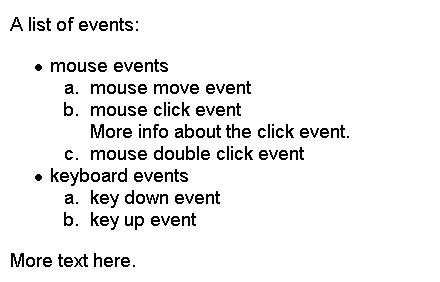
\includegraphics[width= 4 in]{part-basic/chapter-design/pic/design_doc_list.png}
%4.5in
    }
    \caption{事件列表效果\label{pic:design:list}}
\end{figure}

\setitemindent{true}
如果使用~tabs~来缩进,那么要检查~doxygen~配置文件中的
~TAB\_SIZE~设置是否正确。

使用~``.''~可以结束一个列表,并开始一个新的段落。点号
必须与需要对应的~``-''~对齐。这可用于并列多个列表组。
\setitemindent{false}

    \item 使用~HTML~命令

可在文档块中使用~HTML~命令。这样对生成网页更加自然。

    \item 使用~$\backslash$arg~或~@li~命令

可创建简单的非递归的列表。
\end{enumerate}

\subsubsection{高级注释}

高级注释功能包括:
\begin{itemize}
    \item 归组~Grouping
    \item 添加公式
    \item 生成~C++~类层次图
\end{itemize}

具体请查阅相关文档,此处不再赘述。

\subsubsection{例子}

最后给出一个类的文档注释例子。

\clearpage

\ttfamily
\begin{lstlisting}
//!  A test class.
/*!
  A more elaborate class description.
*/
class CTest
{
public:
  //! An enum.
  /*! More detailed enum description. */
  enum TEnum {
        TVal1, /*!< Enum value TVal1. */
        TVal2, /*!< Enum value TVal2. */
        TVal3  /*!< Enum value TVal3. */
    }
    //! Enum pointer.
    /*! Details. */
    *enumPtr,
    //! Enum variable.
    /*! Details. */
    enumVar;

    //! A constructor.
    /*!
      A more elaborate description of
      the constructor.
    */
    CTest();

    /*! \brief A destructor.

      A more elaborate description of
      the destructor.
    */
    ~CTest();

    //! \brief A normal member taking
    //! two arguments and return an integer value.
    /*!
       \param a an integer argument.
       \param s a constant character pointer.
       \return The test results
       \sa CTest(), ~CTest(), testMeToo()
           and publicVar()
    */
    int testMe(int a, const char *s);

    //! A pure virtual member.
    /*!
      \sa testMe()
      \param c1 the first argument.
      \param c2 the second argument.
    */
    virtual void testMeToo(char c1, char c2) = 0;

    //! A public variable.
    /*!
      Details.
    */
    int publicVar;

    //! A function variable.
    /*!
      Details.
    */
    int (*handler)(int a, int b);
};
\end{lstlisting}
\CJKfamily{song}
